\documentclass[fleqn,11pt]{ExcelAtFIT} % Document font size and equations flushed left


%--------------------------------------------------------
%--------------------------------------------------------
%	REVIEW vs. FINAL VERSION
%--------------------------------------------------------

%   LEAVE this line commented out for the REVIEW VERSIONS
%   UNCOMMENT this line to get the FINAL VERSION
%\ExcelFinalCopy


%--------------------------------------------------------
%--------------------------------------------------------
%	LANGUAGE
%--------------------------------------------------------
%   Recommended language for Excel@FIT paper is English.
%   However, in emergency, you can write in Czech or Slovak.
%   In such a case, uncomment one of these lines to localize the template.
%--------------------------------------------------------
%\ExcelSlovakLabels
%\ExcelCzechLabels


%--------------------------------------------------------
%--------------------------------------------------------
%	PDF CUSTOMIZATION
%--------------------------------------------------------

\hypersetup{
	pdftitle={Verification of Pointer Programs Based on Forest Automata},
	pdfauthor={Martin Hruška},
	pdfkeywords={Forest Automata, Formal Verification, Static Analysis, Complex Data Structures, Tree Automata, Backward Run, Predicate Abstraction}
}

\usepackage{comment}
\usepackage{tikz}
\usetikzlibrary{calc,matrix,backgrounds,fit,shapes,arrows}

\newcommand{\vata}[0]{the VATA library}
\newcommand{\Vata}[0]{The VATA library}
\newcommand{\fagr}[0]{\otimes t_1, \ldots, t_n}
\newcommand{\funcdecl}[3]{#1: #2 \rightarrow #3}
\newcommand{\subst}[2]{[#1/#2]} %co, za co
\newcommand{\bexmp}[0]{\noindent\rule{\textwidth}{0.4pt} \begin{example}}
\newcommand{\eexmp}[0]{\end{example} \noindent\rule{\textwidth}{0.4pt}}
\newcommand{\symset}[0]{\mathbb{S}}
\newcommand{\instrset}[0]{\mathbb{I}}
\newcommand{\regs}[0]{\mathbb{G}}
\newcommand{\regsset}[0]{\{r_1, \ldots, r_m\}}
\newcommand{\regssub}[2]{\regs [#1 := #2]}
\newcommand{\regssubmin}[3]{\regs \setminus \{#3\} [#1 := #2]}
\newcommand{\symstate}[3]{(#1, #2, #3)}
\newcommand{\stdsym}[0]{\symstate{F}{\regs}{I}}
\newcommand{\natnum}[0]{\mathbb{N}}

\newcommand{\lfunc}[2]{\lambda #1 \,:\, #2}
\newcommand{\lfuncp}[3]{(\lambda #1 \,:\, #2)(#3)}

\newcommand{\ddispl}[0]{Displ}
\newcommand{\droot}[0]{Root}
\newcommand{\rref}[0]{RR=(\droot,\ddispl)}
\newcommand{\rreftuple}[2]{(#1,#2)}
\newcommand{\rrefreg}[1]{#1=(\droot,\ddispl)}
\newcommand{\ddata}[0]{D = (T,S,V,MB)}

\newcommand{\grev}[0]{g}
\newcommand{\grevinter}[0]{\symset \times \instrset \rightarrow \symset}

\newcommand{\code}[1]{\small{\texttt{#1}}}
\newcommand{\codix}[1]{\emph{\code{#1}}}

\newcommand{\sbwd}[0]{S^{B}_{i}}
\newcommand{\isfwd}[0]{I^{F}}
\newcommand{\sfwd}[0]{S^{F}_{i}}
\newcommand{\ftraceseq}[0]{S^{F}_n \cdots S^{F}_1}
\newcommand{\ftrace}[0]{FT}

\newcommand{\btraceseq}[0]{S^{B}_1 \cdots S^{B}_n}
\newcommand{\btrace}[0]{BT}
\newcommand{\isbwd}[0]{I^{B}}
\newcommand{\bstdsym}[0]{\symstate{F}{\regs}{\isbwd}}


%--------------------------------------------------------
%--------------------------------------------------------
%	ARTICLE INFORMATION
%--------------------------------------------------------

\ExcelYear{2015}

\PaperTitle{Verification of Pointer Programs Based on Forest Automata}

\Authors{Martin Hruška}
\affiliation{*%
  \href{mailto:xhrusk16@stud.fit.vutbr.cz}{xhrusk16@stud.fit.vutbr.cz},
  \textit{Faculty of Information Technology, Brno University of Technology}}
%%%%--------------------------------------------------------
%%%% in case there are multiple authors, use the following fragment instead
%%%%--------------------------------------------------------
%\Authors{Jindřich Novák*, Janča Dvořáková**}
%\affiliation{*%
%  \href{mailto:xnovak00@stud.fit.vutbr.cz}{xnovak00@stud.fit.vutbr.cz},
%  \textit{Faculty of Information Technology, Brno University of Technology}}
%\affiliation{**%
%  \href{mailto:xdvora00@stud.fit.vutbr.cz}{xdvora00@stud.fit.vutbr.cz},
%  \textit{Faculty of Information Technology, Brno University of Technology}}

\Keywords{Forest Automata --- Formal Verification --- Static Analysis --- Complex Data Structures --- Tree Automata --- Backward Run --- Predicate Abstraction}

%\Supplementary{\href{http://youtu.be/S3msCdn3fNM}{Demonstration Video} --- \href{http://excel.fit.vutbr.cz/}{Downloadable Code}}


%--------------------------------------------------------
%--------------------------------------------------------
%	ABSTRACT and TEASER
%--------------------------------------------------------

\Abstract{
  Forest automata are formalism used for analysis and verification of programs manipulating dynamic data structures.
  A~shape analysis related to forest automata has been implemented in Forester tool.
  Forest automata are based on tree automata and Forester has its own implementation of tree automata.
  However, there is the VATA library which implements the efficient algorithms for the tree automata manipulation,
  especially the efficient algorithms for the checking language inclusion of tree automata what is an operation
  crucial also for the verification procedure based on forest automata.
  The first goal of this thesis is to implement a version of Forester tool that uses the VATA library for tree automata manipulation.
  The second goal of this thesis is to extend forest automata based verification with backward run that checks whether
  a found error is a spurious or real one what could be used for refinement of predicate abstraction.
  The first goal has been already fulfill and the variant of Forester using the VATA library participated in the competition SV-COMP 2015.
  The part of the second goal is done only partially since the backward run is already finished and predicate abstraction implementation is
  in progress.
}

%\Teaser{
%	\TeaserImage{placeholder.pdf}
%	\TeaserImage{placeholder.pdf}
%	\TeaserImage{placeholder.pdf}
%}



%--------------------------------------------------------
%--------------------------------------------------------
%--------------------------------------------------------
%--------------------------------------------------------
\begin{document}

\startdocument


%--------------------------------------------------------
%--------------------------------------------------------
%	ARTICLE CONTENTS
%--------------------------------------------------------

%--------------------------------------------------------
%--------------------------------------------------------
%--------------------------------------------------------
%--------------------------------------------------------
\section{Introduction}

The importance of computers in our everyday life has largely increased over the past few decades.
A~lot of us can only hardly imagine doing their jobs without help of an appropriate computer program
and we also spend a plenty of time using computers (e.g. personal computers or mobile devices) in leisure time.
The~computer programs are also often used in very critical instances like autopilot in an airplane.
But the growing number of applications of computer programs brings also need for their greater safety and security.

However, guarantee of software safety and correctness is not an easy task
because the programs often go through many states during computation
and it could be very time and (memory) space demanding or even impossible to check whether no undesirable thing
happens in any of those states.
One approach to ensure software quality is \emph{testing} (and dynamic analysis) which is basically based
on running a program in the different contexts and with the different inputs
and checking whether a program behavior and the outputs are the expected ones.
This method can satisfy many of the requirements for software quality and often cover the great space of the program behaviors
but on the~other side it is only possible to prove presence of the~errors using testing not their absence \cite{dijkstra}.
Moreover finding some errors during testing does not mean that all errors are eliminated.

The mentioned weakness of testing can be resolved by \emph{formal verification}
which is another approach to checking program correctness.
Formal verification is method for checking whether a given system meets a given specification \cite{fav:lecture}.
There are four main branches of formal verification.
The first one is \emph{model checking} which systematically explores the states of a model (e.g. model of a program) to
prove that a property holds along the whole model.
The second approach is \emph{static analysis} which is done over a source code (or some modification of it) of a system
without its explicit execution.
The third approach is \emph{abstract interpretation} where the analysis is performed by
applying abstract transformers corresponding to the original program semantics over an abstract domain.
The last one is \emph{theorem proving}.
It proves the program in a standard mathematical way -- starting from axioms and proving theorems to
verify the properties of a given system.
Theorem proving could be partially automated.

This work deals with a specific part of static analysis called \emph{shape analysis} which is focused on the verification of the programs manipulating
complex data structures (like the different kinds of lists and trees), typically allocated on the heap.
The properties checked for this class of programs are for example checking whether no dangling
pointers are dereferenced (no invalid dereferences), whether all allocated memory on a heap is also freed (no memory leaks)
during the program execution or whether there is not freed pointer which has no assigned memory (no invalid free).
There are different approaches to this kind of static analysis with the different advantages.
For example, the approach based on \emph{separation logic} \cite{seplog,seplog07} provides scalability of a verification procedure.
On the other side, the automata based approach, particularly \emph{abstract tree regular model checking} (ATRMC) \cite{artmc}, is
superior in its flexibility.
However, this thesis is focused on a verification procedure based on a concept of forest automata (FA) which
combines benefits of the both mentioned approaches.

Forest automata has been introduce in \cite{forester11,forester12} and they are an extension of finite automata or more precisely extension of finite tree automata (TA).
They are used as an abstract domain in related verification procedure over which a symbolic execution of a analyzed program is performed.
A~prototype of this verification procedure has been implemented in a tool called \emph{Forester}.
Forester verifies programs written in C language and it can detect invalid dereferences, invalid free, memory leaks and also reachability of an error label.
It is yet able to verify non-trivial data structures like the skip-lists of the second and the third level
but there is still a room for its improvement.
E.g. Forester currently does not support complete C language syntax and
it is not also yet possible to check whether a found error is real or spurious.
It is also needed to refactore some parts of Forester code before an extension of the tool.
A~general goal of this thesis is improving Forester in the areas described further.


Since FA are highly related to the finite tree automata the first of the goals of the thesis is to implement
a version of Forester using \vata\ -- state-of-the-art library for TA manipulation \cite{libvata}.
Particularly, this consists creating an interface between Forester and VATA to employ VATA as a TA library for Forester backend
which should bring better maintainability and modularity then implement a special TA library inside Forester as it is now.
The second goal of this thesis is to design and implement \emph{backward run} for FA based verification
which enables checking spuriousness of an error found in a program.
The error could be spurious because too high abstraction over FA is used.
The information gained by backward run could be used for the refinement of \emph{predicate abstraction} (one kind of abstraction over FA)
to prevent verification procedure from getting the same spurious error again.
However, Forester does not use predicate abstraction but \emph{height abstraction} now
because predicate abstraction needs the backward run.
Height abstraction is less precise and less flexible compared to predicate abstraction so implementing predicate abstraction
enables analysis of even more complex data structures like the red-black trees.
A~part of the second goal is just completing and testing implementation of backward run and predicate abstraction in Forester.

This paper is structured as follows.
In Section \ref{sec:overview} a high level overview of shape analysis based on forest automata
is given.
Then the closer description of backward run and predicate abstraction is introduced in Section \ref{sec:br}.
Section \ref{sec:forvata} provides description of modification of Forester to use the VATA library as a backend.
Finally, conclusions of the work takes a place in Section \ref{sec:concl}.

%--------------------------------------------------------
%--------------------------------------------------------
%--------------------------------------------------------
%--------------------------------------------------------
\section{High Level Overview}
\label{sec:overview}

\begin{figure}[t]
	\centering
	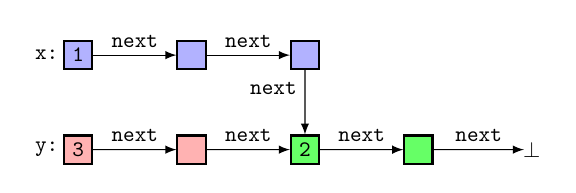
\begin{tikzpicture}[
  scale=0.8,
  transform shape,
]

  \tikzstyle{memnode}=[draw,rectangle,fill=lightgray,thick,minimum height=4.5mm, minimum width=4.5mm,inner sep=1mm,node distance=18mm,font=\tt]
  \tikzstyle{memnodeblue}=[draw,rectangle,fill=blue!30,thick,minimum height=4.5mm, minimum width=4.5mm,inner sep=1mm,node distance=18mm,font=\tt]
  \tikzstyle{memnodepink}=[draw,rectangle,fill=red!30,thick,minimum height=4.5mm, minimum width=4.5mm,inner sep=1mm,node distance=18mm,font=\tt]
  \tikzstyle{memnodegreen}=[draw,rectangle,fill=green!60,thick,minimum height=4.5mm, minimum width=4.5mm,inner sep=1mm,node distance=18mm,font=\tt]

  \tikzstyle{nullnode}=[node distance=18mm,label=center:$\bot$]
  \tikzstyle{varnode}=[font=\tt]
  \tikzstyle{refnode}=[fill=green!20,minimum height=4.5mm, minimum width=4.5mm,inner sep=1mm,font=\tt]

  \tikzstyle{pointer}=[draw,->,>=latex]
  \tikzstyle{ptrlab}=[above,font=\tt]

  % nodes
  \node[memnodeblue] (x1) at (0mm,0mm) {1};
  \node[memnodeblue] (x2) [right of=x1] {};
  \node[memnodeblue] (x3) [right of=x2] {};

  \node[memnodepink] (y1) [below of=x1, yshift=3mm] {3};
  \node[memnodepink] (y2) [right of=y1] {};

  \node[memnodegreen] (join) [right of=y2] {2};
  \node[memnodegreen] (j2) [right of=join] {};
  \node[nullnode] (j2null) [right of=j2] {};

  \node[varnode,node distance=5mm] (x) [left of=x1] {x:};
  \node[varnode,node distance=5mm] (x) [left of=y1] {y:};

  % pointers
  \draw[pointer] (x1)    -- node[ptrlab]   {next} (x2);
  \draw[pointer] (x2)    -- node[ptrlab]   {next} (x3);
  
  \draw[pointer] (x3)    -- node[ptrlab,xshift=-5mm]   {next} (join);

  \draw[pointer] (y1)    -- node[ptrlab]   {next} (y2);
  \draw[pointer] (y2)    -- node[ptrlab]   {next} (join);

  \draw[pointer] (join)  -- node[ptrlab]  {next}     (j2);
  \draw[pointer] (j2)    -- node[ptrlab]  {next}     (j2null);

\end{tikzpicture}

	
	\vspace{0.5cm}
	
	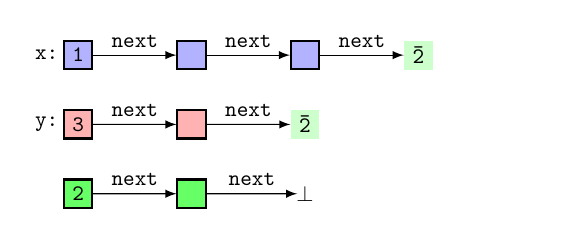
\begin{tikzpicture}[
  scale=0.8,
  transform shape,
  node distance=18mm
]

  \tikzstyle{memnode}=[draw,rectangle,fill=lightgray,thick,minimum height=4.5mm, minimum width=4.5mm,inner sep=1mm,node distance=18mm,font=\tt]
  \tikzstyle{memnodeblue}=[draw,rectangle,fill=blue!30,thick,minimum height=4.5mm, minimum width=4.5mm,inner sep=1mm,node distance=18mm,font=\tt]
  \tikzstyle{memnodepink}=[draw,rectangle,fill=red!30,thick,minimum height=4.5mm, minimum width=4.5mm,inner sep=1mm,node distance=18mm,font=\tt]
  \tikzstyle{memnodegreen}=[draw,rectangle,fill=green!60,thick,minimum height=4.5mm, minimum width=4.5mm,inner sep=1mm,node distance=18mm,font=\tt]

  \tikzstyle{nullnode}=[node distance=18mm,label=center:$\bot$]
  \tikzstyle{varnode}=[font=\tt]
  \tikzstyle{refnode}=[fill=green!20,minimum height=4.5mm, minimum width=4.5mm,inner sep=1mm,font=\tt]

  \tikzstyle{pointer}=[draw,->,>=latex]
  \tikzstyle{ptrlab}=[above,font=\tt]

  % nodes
  \node[memnodeblue] (x1)  at (0mm,0mm) {1};
  \node[memnodeblue] (x2) [right of=x1] {};
  \node[memnodeblue] (x3) [right of=x2] {};

  \node[memnodepink] (y1) [below of=x1, yshift=7mm] {3};
  \node[memnodepink] (y2) [right of=y1] {};

  \node[refnode] (joinsbst1) [right of=x3] {\=2};
  \node[refnode] (joinsbst2) [right of=y2] {\=2};

  \node[memnodegreen] (join) [below of=y1, yshift=7mm] {2};
  \node[memnodegreen] (j2) [right of=join] {};
  \node[nullnode] (j2null) [right of=j2] {};

  \node[varnode,node distance=5mm] (x) [left of=x1] {x:};
  \node[varnode,node distance=5mm] (x) [left of=y1] {y:};
  
  \node (placeholder) [right of=joinsbst1] {};
  

  % pointers
  \draw[pointer] (x1)    -- node[ptrlab]   {next} (x2);
  \draw[pointer] (x2)    -- node[ptrlab]   {next} (x3);
  \draw[pointer] (x3)    -- node[ptrlab]   {next} (joinsbst1);

  \draw[pointer] (y1)    -- node[ptrlab]   {next} (y2);
  \draw[pointer] (y2)    -- node[ptrlab]   {next} (joinsbst2);

  \draw[pointer] (join)  -- node[ptrlab]   {next} (j2);
  \draw[pointer] (j2)    -- node[ptrlab]   {next} (j2null);

\end{tikzpicture}

	\caption{
	Figure shows tree decomposition of a heap graph.
    The heap graph representing singly-linked list is shown in the top of Figure.
	The nodes could be labeled by a pointer variable that references allocated memory cell
	corresponding to the node.
	Moreover the cut-points are labeled by a number that they have in ordering over
	the cut-points.
	In this case there are three cut-points with order $1$, $2$ and $3$.
	The graph is split to the three trees shown in the bottom of Figure during the heap decomposition.
	The new trees could contain the references to another trees, in this case tree $1$ and tree $3$
	have the nodes referencing tree $2$.}
	\label{fig:graph}
\end{figure}

This section provides a high level overview of the verification procedure based
on forest automata.
As it was already mentioned we consider C programs manipulating dynamic data structures.
The simple examples of such structures are a singly-linked list or a binary tree.
Consider a singly-linked list containing an (integer) data member and a pointer
to the next item in the list and also
consider two variables $x,y$ pointing the singly-linked list.
An instance of the singly-linked list allocated on a heap could be viewed as an oriented graph.
The nodes of the graph correspond to the allocated memory cells
and the edges of the graph are related to the pointers referencing
another allocated memory cell of the list.
Each node could be labeled by a name of the pointer variables that
reference the given node or it could be labeled by a data contained in the node.
The example of such a graph is shown in~Figure~\ref{fig:graph}.
We ommit the data nodes in Figure \ref{fig:graph} for sake of clarity.
The figure shows that the variables $x$, $y$ points two singly-linked list (the blue and the red nodes) that
have common part (the green nodes).
The original heap graph is shown in the top of Figure \ref{fig:graph}.
The tree decomposition, which is decribed later, is in the bottom of Figure \ref{fig:graph}.

We can decompose the graph to a set of trees by the following method.
First we identify so called \emph{cut-points} what are the nodes referenced by
one or more pointer variables or the nodes having more than one incoming edges.
The cut-points are then numbered by a depth-first traversal of the graph that starts from
the nodes referenced by the pointer variables.
The graph at Figure \ref{fig:graph} has the three cut-points that are labeled by the numbers $1$,
$2$ and $3$ what denotes the node order in the cut-points ordering.
Then the graph is split to the trees with cut-point as the roots.
The new trees do not contain no cut-points.
At Figure \ref{fig:graph} the graph graph to the trees is shown at the bottom.
Finally, we need to take care of is redirecting the edges, which lead to the nodes
marked as the cut-points, to the new nodes because the cut-point are now roots of trees and
so cannot have the incoming edges.
The new nodes replacing cut-points are labeled by a number referencing to the tree that has a related cut-point like a root.
The example at Figure \ref{fig:graph} shows that tree $1$ and tree $3$ contains the nodes with label $\overline{2}$
referencing tree~$2$.

The set of trees (created by graph decomposition) is called forest.
Such a forest could be accepted by a forest automaton.
A~forest automaton is a tuple of finite tree automat which are automata accepting trees instead of words (in comparsion with finite automata).
The tree automata within a forest automaton are interconnected by references (that are also symbols in their alphabet)
so we are able to accept the forests representing state of heaps by forest automata.

So far we are described how to represent dynamic data structures by forest automata.
They can be viewed also as an abstract domain in context of abstract interpretation
whereas a concrete domain is a set of heaps.
It is also possible to define abstract transformers corresponding to the (concrete) program operations over forest automata.
The verification procedure is then possible to perform as a symbolic execution
where abstract transformers are gradually applied to abstract domain.
When an error like a invalid memory reference or invalid free happens during the symbolic
execution it implies that it is possible that there is an error in the program (but because
the forest automata overapproximate the state space of the original program the error could be spurious).

It is possible to represent a dynamic data structure with bounded number of cut-points.
But there are data structures like a doubly-linked list where each node is a cut-point because
it is pointed by the next and also previous member of the list.
This could lead to the unbounded number of cut-points.
It possible to resolve this problem by introducing so-called \emph{boxes}.
The repeating sub-graphs causing unboudness of cut-points are collected to boxes.
Then these sub-graphs are replaced by hyperedge labeld by an appropriate box.
This transformation changes graph to a new hiearchical hypergraph with bounded number of boxes.
It is still possible to decompose either hypergraph or boxes to the tree components in the way
described above.
So it is also represent the hypergraph with forest automata.
This forest automata should be also hiearchical as the graphs are, beucase they
should include forest automata of lower level representing boxes in their alphabet.
The nesting of forest automata to symbols of alphabet of forest automata of higher level
could be done in more levels so we get real hierarchy.

More technical details about a heap decomposition and forest automata could be found in \cite{forester11, forester13}.

\section{Backward Run and Predicate Abstraction}
\label{sec:br}

\begin{figure}[t]
	\centering
	
\includegraphics[width=0.7\linewidth]{keep-calm.png}
	\caption{Good writing is bad writing that was rewritten several times.  Don't worry, start somewhere.}
	\label{fig:KeepCalm}
\end{figure}

We described how to represent dynamic data structures by forest automata.
The forest automata make us able to handle also infinite state spaces
rising from the unboundness of the mentioned dynamic data structures.
However, the state explosion could still occur what lead
to nearly impossibility of finish verification procedure in real time.
Therefore the abstraction over the forest automata is introduced.
The abstraction accelerates the computation by merging more states
of forest automata to one abstract state.
The negative effect of the abstraction is the overapproximation of the reachable
states of an analyzed system.
In the case of computer programs this leads to finding reachable error states in
abstracted state space which are not present in real system.
This could be prevented by a refinement of the abstraction
which prevent the abstraction to include the part of state space where
the spurious error has been example.

Forester now contains a height abstraction.
This abstraction merges states whose languages (language of state is set of trees) are the same
when the trees of the language are compared only to the given depth.
The main problem of this abstraction technique is its scalability because
the only one way how to scale it is by the parameter defining the depth of tree comparison.
The more precise abstraction is so called \emph{predicate abstraction} that introduces
set of predicates and merges the states in which the same predicates hold.
When a spurious counterexample is found, then the set of predicates is extended by
a predicate that prevents reaching the spurious counterexample again
and the verification procedure is rerun again with the new predicate.

Finding the new predicate and checking spuriousness of an error is done by performing of \emph{backward run}.
A~backward run starts from forest automata modelling a heap with spurious error and
reverting gradually each abstract operation over the forest automata
in backward order.
When an automata with empty language is get by intersection between forest automata
get from the backward run and forward run is yield then the error is spurious.
The automaton modelling the last non empty intersection of forward and backward run
is then used like a new predicate.

Forester implementation of abstract transformers does not modify
forest automata at all.
It often performs just some changes in symbolic state not
affecting forest automata so it is possible to revert these operations without
need of performing of intersection of forest automata to get previous backward
run symbolic state.
However, there are critical operations like freeing a memory node that the intersection
needs.

The goal of this work is to implement backward run and the predicate abstraction
for non-hierarchical forest automata.
It includes design of the reverse operations for abstract transformers over
the abstract domain and the application of predicate abstraction to forest automata.
Morever, in the reverse operations the intersection of foster automata is needed
so it is also part of this work to implement it.
Forester has some basic implementation of both, the reverse microcode instructions and
intersection of forest automata.
However, the implementation was not mature enough so it was necessary to
complete it and evaluate it on the SV-COMP benchmark.

The implementation of the backward run has been already finished
and evaluate on the benchmark.
The results are in Table \ref{Tab:bwres}.
The implementation helps in identifying of the X spuriousness counterexamples and
confirmation of Y real errors.
The test cases with a spurious counterexamples will be further resolved by implementing predicate
abstraction which is currently in progress.

This work however does not contain backward run and predicate abstraction over
the programs where hiearchical forest automata because the forest automata unfolding
would be needed for implementing intersection in these cases
what is exceed room of this work.
But it would be a great space for future work.

\begin{table}[h]
	\vskip6pt
	\caption{Table of Grades}
	\centering
	\begin{tabular}{llr}
		\toprule
		\multicolumn{2}{c}{Name} \\
		\cmidrule(r){1-2}
		First name & Last Name & Grade \\
		\midrule
		John & Doe & $7.5$ \\
		Richard & Miles & $2$ \\
		\bottomrule
	\end{tabular}
	\label{tab:ExampleTable}
\end{table}


\section{Forester and VATA}
\label{sec:forvata}

This section describes how Forester has been refactored to be able to employ \vata\ 
efficient implementation of	tree automata and the operations over them,
especially checking inclusion of languages of tree automata.
Forester had its own implementation of tree automata (in module called TA) and their operations
but it is not as efficient as VATA is and it is also less maintable
then using the library that implements state-of-the-art algorithms.

VATA provides two encodings of tree automata -- explicit and semi-symbolic.
They differs mainly in a way of representation of transition relation of tree automata.
The explicit encoding stores the transitions in an explicit hash tables while the semi-symolic
uses a multi binary decision diagram.
We use the implementation of explicit encoding of TA in this work because
it is currently the only one that support the most of needed operations over TA and it is also more efficient than
semi-symbolic encoding for the purposes of Forester because no large alphabets are used during the verification procedure
so the advantage of the semi-symbolic encoding would not be fully utilized here.

Forester implementation is currently far from being mature and
high structural dependencies is one of its bottlenecks.
So the first thing needed to be done was reducing number of dependencies between classes,
especially reduction of dependencies to the existing Forester module implementing tree automata.
One of approaches how to do this is applying \emph{Law of Demeter} \cite{lod89} to the code manipulating tree automata what practically
means that classes using TA explicitly should implement methods providing information about TA instead of providing instance of TA object itself.
Applying the Law of Demeter reduces knowledge needed about implementation of TA module across the whole project.
Another way of reducing structural dependencies is making all possible methods and members of TA (in sense of C++ language \cite{stroustrup13}).
This creates an explicitly tight interfaces to tree automata module so it is easier to see which methods needs to implement
a new tree automata implementation.
The last from the most used techniques of refactoring is employing \emph{auto} type deduction in C++ in combination
with the \emph{Iterator} pattern.
It is used for example when one needs to iterate over all transitions of tree automata or all transitions which
have same state as parent.

After refactoring it is possible to apply design pattern \emph{adapter} \cite{gamma95} to create
an interface between Forester and \vata.
Applying the adapter design pattern makes possible to include VATA without need of rewriting
Forester to the~names of methods and data members used in VATA.
It creates also only one place (particularly adapter class) connecting Forester and VATA instead of
including VATA into many of the Forester classes and so it prevents from creating too strong relation between them.

The main part of the adapter patter is in our case newly implemented class \emph{VATAAdapter} playing role of Adaptor.
We decided to used the implementation approach to Adaptor, preferring composition over inheritance.
It is more suitable for our purposes since we often needs to rename methods 
(a name of a method in Forester differs from a name of a method in VATA performing the same operation)
or convert a data type of parameter of tree automata operation (e.g. from vector to set). 

Now we provide more technical details about implementation of the adapter pattern.
The class \emph{VATAAdapter} instantiates class \emph{ExplicitTreeAut} from VATA as its private data member
and redirects to this instance method calls from Forester (the names of methods of VATAAdapter are the same as they were
in the original Forester TA library).
\emph{VATAAdapter} also sometimes performs mentioned conversion of the data types.
There are methods implemented by adapter not presented in VATA like method \emph{unfoldAtRoot}
performing an unfolding, an operation specific for forest automata.
The methods of this kind are very Forester specific so it is not sensible to add them to general purpose library like VATA is
and it is better to implement them in interface like class VATAAdapter is.

We originally supposed that it would be possible to keep the original TA module along VATA adapter
to be able to easily switch between them.
However it has shown that this would bring high overhead in some situations.
E.g., a~conversion of some data types would be needed in this case
what is overhead compared to implementation where data types compatible with VATA are used directly in the Forester code.
Hence we decided to remove the original tree automata module and further support only version of Forester with \vata.

%--------------------------------------------------------
%--------------------------------------------------------
%--------------------------------------------------------
%--------------------------------------------------------
\section{Conclusions}
\label{sec:concl}

The main goals of this thesis were (a) to implement version of Forester tool that uses the VATA library for tree automata representation and manipulation
and (b) to extend verification procedure based on forest automata with backward run for detection of the spurious errors found in the analysed program.
The theory of forest automata and related theory of tree automata has been studied and described in this thesis and the verification procedure
based on forest automata has been also explored to fulfill the thesis goals.
The connection of Forester and \vata\ was designed and implemented after the analysis of the both tools.
Forester had to be refactored for this purposes.

The first goal has been already reached and the version of Forester using the VATA library successfully participated in competition SV-COMP 2015 \cite{www:svcomp}.
The second goal is partly finished.
The backward run with needed forest automata intersection for non-hiearchical forest automata has been completed and evaluated on SV-COMP benchamark.
The implementation of predicate abstraction is currently in progress.

The future work after finishing the basic predicate abstraction could be in generalizing the method to the hiearchical forest automata
what enables Forester to analyze more test cases.
Forester code needs also to further refactored and also greater support for C language construction should be added to be
able to analyse more real work programs.
The mentioned work should help Forester to win SV-COMP 2016 competition.
%\textbf{[Highlights of Results]} Particular numbers. Remind the reader that the paper matters.
%\phony{Lorem ipsum dolor sit amet, consectetur adipiscing elit. Sed tempus fermentum ipsum at venenatis. Curabitur ultricies, mauris eu ullamcorper mattis, ligula purus dapibus mi, vel dapibus odio nulla et ex. Sed viverra cursus mattis. Suspendisse ornare semper condimentum. Interdum et malesuada fames ac ante ipsum.}

%\textbf{[Paper Contributions]} What is the original contribution of this work? Two or three thoughts that one should definitely take home.
%\phony{Lorem ipsum dolor sit amet, consectetur adipiscing elit. Praesent posuere mattis ante at imperdiet. Cras id tincidunt purus. Aliquam erat volutpat. Morbi non gravida nisi, non iaculis tortor. Quisque at fringilla neque.}

%\textbf{[Future Work]} How can other researchers / developers make use of the results of this work?  Do you have further plans with this work? Or anybody else?
%\phony{Lorem ipsum dolor sit amet, consectetur adipiscing elit. Suspendisse sollicitudin posuere massa, non convallis purus ultricies sit amet. Duis at nisl tincidunt, maximus risus a, aliquet massa. Vestibulum libero odio, condimentum ut ex non, eleifend.}


%--------------------------------------------------------
%--------------------------------------------------------
%--------------------------------------------------------
%	REFERENCE LIST
%--------------------------------------------------------
%--------------------------------------------------------
\phantomsection
\bibliographystyle{unsrt}
\bibliography{2015-ExcelFIT-ShortName-bib}

%--------------------------------------------------------
%--------------------------------------------------------
%--------------------------------------------------------


%--------------------------------------------------------
%--------------------------------------------------------
%--------------------------------------------------------
%--------------------------------------------------------
\begin{comment}
\section{How To Use This Template}
\label{sec:HowToUse}

Here will go several sections describing \textbf{your work}. From theoretical background (Section 2), through your own methodology (Section 3), experiments and implementation (Section 4 and possibly 5), to conclusions (Section 6). Instead of such technical content, here in this template we give a few hints how to write the paper.

\begin{figure}[t]
	\centering
	
\includegraphics[width=0.7\linewidth]{keep-calm.png}
	\caption{Good writing is bad writing that was rewritten several times.  Don't worry, start somewhere.}
	\label{fig:KeepCalm}
\end{figure}

Here is a list of actions to do first when you want to write an Excel@FIT paper:
\begin{enumerate}
	\item Download all the template files (Sec.~\ref{sec:FilesInTemplate}) into a directory. Maybe setup a GIT sync for backup, sharing, and for use from multiple computers.
	\item Rename \textit{2015-ExcelFIT-ShortName.tex} -- replace ShortName with something that identifies your work and is short enough.  For example: \textit{VehicleBoxes}, \textit{VanishingPoints}, \textit{FastShadows}, \textit{NewProbeTesting}, \textit{CheapDynamicDNS}, \ldots  This ensures that the filename already gives a hint what is in there (\textit{mypaper.pdf} is really stupid).
	\item Insert meta information: \textbf{your name}, \textbf{e-mail}, \textbf{paper title}.  Make sure the year in the top right corner of the document is correct.  Do not hesitate to use ěščřžýáíé in your name -- the \LaTeX{} template is configured to eat UTF8 Unicode.
	\item Insert teaser images (``image abstract'').  Use as many \textit{$\backslash$TeaserImage} commands as suitable -- three or four will usually be fine for a one-line teaser.  If you absolutely don't have any image showing your work (what kind of work could that be, anyway?!), remove the \textit{$\backslash$Teaser} command.
	\item Insert references to supplementary material.  That will typically be clickable links to a youtube / vimeo video and to downloadable code, hyperlink to an online demo, or a github repo. If you have anything else relevant, put it in.  If there is no supplementary material (really?!), remove or comment out the \textit{$\backslash$Supplementary} command.
	\item Keep calm and start writing (Figure~\ref{fig:KeepCalm}).  Some suggestions how to do this are in Section~\ref{sec:HowToWrite}.
	\item When your paper is accepted to Excel@FIT, uncomment \textit{$\backslash$ExcelFinalCopy} at the beginning of this file.  The line numbers will disappear from the sides of the text and your paper is ready for final publication.
\end{enumerate}

Jean-Luc Lebrun \cite{Lebrun2011} offers excellent recommendations for the canonical sections of scientific/technical papers.  That is why Abstract, Introduction, and Conclusions in this template are already structured.  This structure is no more than a recommendation, but divert from it only in cases when you exactly know what you are doing.  The ``phony'' texts (typeset in \phony{gray color}) roughly indicate the lengths of individual parts of these sections.  Replace them with reasonable amounts of text.

%--------------------------------------------------------
%--------------------------------------------------------
\subsection{What Files are Here and Why}
\label{sec:FilesInTemplate}

The template package for Excel@FIT papers contains these files:
\begin{description}[noitemsep]
	\item[2015-ExcelFIT-ShortName.tex] This is the template for the main \LaTeX{} file -- this is your paper.  It might be a good idea to put each section to an individual file as mentioned before.  Do yourself a favor and replace \textit{ShortName} in the filename with something meaningful.
	\item[2015-ExcelFIT-ShortName-bib.bib] You can erase the contents of this file completely and start adding BibTeX references.  It is much easier to use a small editing tool (Section~\ref{sec:UsefulTools}, JabRef) than to format \textit{.bib} file manually.  Rename the file so that \textit{ShortName} is consistent with the previous file (and update the filename in the \textit{.tex} file).
	\item[ExcelAtFIT.cls] \LaTeX{} class file based on the \emph{Stylish Article}%
	  \footnote{\url{http://www.latextemplates.com/template/stylish-article}} document class.  Do not modify this file.
	\item[ExcelAtFIT-logo.pdf] This is the logo on the title page.
	\item[images/placeholder.pdf] Placeholder image; include it, scale it as needed, then replace it with real content.\\ 
\includegraphics[height=4em]{placeholder.pdf}
	\item[images/keep-calm.png] You don't need this file; it's only used in this template to show how to include a \textit{.png} file (Figure~\ref{fig:KeepCalm}).
\end{description}

%--------------------------------------------------------
%--------------------------------------------------------
%--------------------------------------------------------
%--------------------------------------------------------
\section{How To Write the Paper --- A~Few Hints}
\label{sec:HowToWrite}

A~reasonable way to start writing is sketching the \textbf{abstract} \cite{Herout-Abstract}.  Writing the abstract helps focus on what is important in the paper, what is the contribution, the meaning for the community.  This exercise might take some 20 minutes and it pays back by clearing the key points of the text.  
In 99\,\% cases it is very reasonable to stick to the abstract structure \cite{Lebrun2011} which is provided in this template.

Once you have the abstract, it should be very clear what is the message of the paper, what is the newly introduced knowledge, what are the proofs of its contribution, etc.  This is the right time to start constructing the \emph{skeleton} of the paper: it's \textbf{comics edition}~\cite{Herout-Comics}.
This thing is composed of mainly four items:
\begin{enumerate} [noitemsep]
	\item \textbf{Sections and subsections.}
	\item \textbf{Figures and tables.}  At this phase, knowing that ``once there will be a figure about this and that'' is just fine.  That is why we have the \textit{placeholder.pdf} image -- see Figure~\ref{fig:WidePicture}.  If this totally generic image can be replaced by some temporary image which still needs more work, but which is closer to the target version, go ahead. A~hand-drawing photographed by a cellphone is perfect at this stage.
	\item \textbf{Todo's.} In the early comics version, every section is filled by one or more \texttt{$\backslash$todo} commands and nothing else.  A~todo in the text might look like: \todo{you should do something}.  Unlike some elaborated todo packages, this simple solution (defined in the template) does not break the page formatting and it is perfectly sufficient.
	\item \textbf{Phony placeholder texts.}  These help you estimate the proportions of individual sections and subsections and to better aim at the correct paper length. Use \textit{$\backslash$blind\{3\}} to get three paragraphs of beautiful \phony{grey phony text}.
\end{enumerate}
One hour is usually enough for creating a nice comics edition of the paper.  No reason to wait, make a copy of the template and start butchering it. 

Having the comics edition usually lubricates the whole writing process.  Now, the paper contains 20 or so todo's -- why not take the easiest one of them and replace it with a few lines of text within 15 minutes or even less.  Writing is no more a scary complex work.

%--------------------------------------------------------
%--------------------------------------------------------
\subsection{Images and Tables}
\label{sec:Images}

Visuals (figures, tables, good equations, section headings) make the skeleton of a properly written paper.  A~time-stressed reader should be able to get the idea from only browsing them.  
Therefore:
\begin{enumerate}[noitemsep]
\item \textbf{Make them perfect.}  Cheap and ugly images -- cheap and ugly paper.  Imperfect or shorter text -- who cares?
\item \textbf{Make them self-contained.}  Be not afraid to have a ten-lines-long caption under an image.  The image plus its caption must make perfect sense by themselves, without reading the text.
\item \textbf{Make them many.}  EVERY technical idea is better explained by an image.  Two images per page are a moderate start.
\end{enumerate}
\LaTeX{} lets you easily insert both vector and raster graphics. It is reasonable to use three formats:
\begin{description}[noitemsep]
\item[.pdf] Perfect for vector graphics.  All graphs \textbf{must} be in vector and therefore in .pdf.  Gnuplot, pyplot, Matlab -- they all produce vector graphs in .pdf easily.  Diagrams, system structures, sketches -- all vector graphics.  It's 2015, not 1980 anymore\ldots
\item[.jpg] Suitable for photos.  \textbf{Never} for plots or screenshots.
\item[.png] Good for precise raster graphics.  Screenshots, raster plots, raster outputs of programs.  Not for diagrams and plots -- unless it is a one-in-ten-years exception.
\end{description}
Caption of a table goes \textbf{before} the table (e.g. Table~\ref{tab:ExampleTable}), just the opposite way than with figures.  There is no logic behind, that's just how it is.

%--------------------------------------------------------
%--------------------------------------------------------
\subsection{Sections and Subsections}
\label{sec:Sections}

It is usually wrong to have subsections in the Introduction; it is always wrong to have them in Conclusions.  In this kind of paper, it is very likely to be wrong to have any subsubsections.

Section headings are the skeleton of the paper -- make them accurate and descriptive.  One-word section titles (apart from Introduction and Conclusions) are typically wrong, because they are not descriptive.  
``Proposed Method for Running X by Using Y'' is better than ``The Method''.
``Implemented Application for PQR Communication'' is better than ``Application''.  The outline of all section titles should contain all the keywords relevant for the work.  Just by seeing them, the reader should be able to tell precisely the topic of the paper.  If not, the section headers are wrong (usually too short and generic).

%--------------------------------------------------------
%--------------------------------------------------------
\subsection{Keywords}
\label{sec:Keywords}

Keywords are specified at the top of the document.  
\begin{enumerate}[noitemsep]
	\item When making the list of keywords, ask yourself this: ``What should one write to google, so that the right answer would be my paper?''
	\item Very generic terms (``IT'', ``Graphics'', ``Hardware'') are useless. Narrow terms are fine (``Matrix Code Recognition'', ``Appearance-Based Vehicle Segmentation'', \ldots)
\end{enumerate}

%--------------------------------------------------------
%--------------------------------------------------------
%--------------------------------------------------------
%--------------------------------------------------------
\section{Some Useful Tools}
\label{sec:UsefulTools}

This list is not a list and it is by no means complete.  If you prefer other tools -- cool, stick with them.  If you are just beginning, consider these.

\begin{description}
	\item[\href{http://miktex.org/download}{MikTeX}] Problem-free \LaTeX{} for Windows; a distribution with perfect automation of package download. Single setup, no more worries.
	\item[\href{http://texstudio.sourceforge.net/}{TeXstudio}] Portable and opensource GUI for \LaTeX{} writing.  Ctrl+click jumps from pdf to latex and back.  Integrated spellchecker, syntax highlighting, multifile projects, etc.  First, install MikTeX, then TeXstudio.  Ten minutes and you are a \LaTeX{} master.
	\item[\href{http://jabref.sourceforge.net/download.php}{JabRef}] Nice and simple Java program for managing \textit{.bib} files with references.  Not much to learn -- one window, a straightforward form for editing the entries.
	\item[\href{https://inkscape.org/en/download/}{InkScape}] Opensource and portable editor of vector files (SVG and -- conveniently -- PDF).  The proper tool for making great drawings for papers -- not the easiest to learn, though.
	\item[GIT] Great for team collaboration on \LaTeX{} projects, but also helpful to a single author -- for versioning, backup, multi-computer, \ldots
	\item[\href{http://www.overleaf.com/}{Overleaf}] Online \LaTeX{} editing -- some love it, to others it might seem a little too slow, though\ldots
\end{description}


%--------------------------------------------------------
%--------------------------------------------------------
%--------------------------------------------------------
%--------------------------------------------------------
\section{Frequently Used \LaTeX{} Fragments}
\label{sec:Fragments}

Here goes an example of a table:
\begin{table}[h]
	\vskip6pt
	\caption{Table of Grades}
	\centering
	\begin{tabular}{llr}
		\toprule
		\multicolumn{2}{c}{Name} \\
		\cmidrule(r){1-2}
		First name & Last Name & Grade \\
		\midrule
		John & Doe & $7.5$ \\
		Richard & Miles & $2$ \\
		\bottomrule
	\end{tabular}
	\label{tab:ExampleTable}
\end{table}

Figure~\ref{fig:WidePicture} shows a wide figure, Figure~\ref{fig:KeepCalm} is a single-column figure with width specified relatively to the column.
\begin{figure*}[t]\centering % Using \begin{figure*} makes the figure take up the entire width of the page
  \centering
  
\includegraphics[width=0.8\linewidth,height=1.7in]{placeholder.pdf}\\[1pt]
  
\includegraphics[width=0.2\linewidth]{placeholder.pdf}
  
\includegraphics[width=0.2\linewidth]{placeholder.pdf}
  
\includegraphics[width=0.2\linewidth]{placeholder.pdf}
  
\includegraphics[width=0.2\linewidth]{placeholder.pdf}
  \caption{Wide Picture.  The whole figure can be composed of several smaller images.  If you want to address individual images in the caption or from the text, use the \textit{subcaption} package.}
  \label{fig:WidePicture}
\end{figure*}
Some mathematics $\cos\pi=-1$ and $\alpha$ in the text%
\footnote{And some mathematics $\cos\pi=-1$ and $\alpha$ in a footnote.}.

Now, this is an equation:
\begin{equation}
\cos^3 \theta =\frac{1}{4}\cos\theta+\frac{3}{4}\cos 3\theta
\label{eq:refname2}
\end{equation}
and here is a bunch of equations aligned horizontally:
\begin{align}
	3x &= 6y + 12 \\
	x &= 2y + 4
\end{align}

\blind{1}
\end{comment}

\end{document}
